%\title{Building Perfect Brackets}

\documentclass[5p, preprint]{elsarticle}
 
\usepackage{cite}

\usepackage[cmex10]{amsmath}
\usepackage[parfill]{parskip}
\usepackage{url}
\usepackage{graphicx}
\usepackage{subfig}
\usepackage{caption}

% correct bad hyphenation here
\hyphenation{op-tical net-works semi-conduc-tor}


\begin{document}

\title{Building Perfect Tournament Brackets with Data Analytics}

\author{Christopher D. Hagmann\fnref{fn1}}
\ead{chagmann@purdue.edu}

\author{Nan Kong\fnref{fn2}}
\ead{nkong@purdue.edu}


\begin{abstract}
The NCAA men's basketball tournament highlights data analytics to the everyday person as they look for help building their brackets. A k-Nearest Neighbors algorithm is proposed to compare new opponents to previously played teams. A distance between teams is calculated to determine the most similar teams and to weigh the value of each win or loss to the teams. The value of k is determined from previous years and applied to 2014. Results are compared to other predictions for 2014.
\end{abstract}

% Note that keywords are not normally used for peerreview papers.
\begin{keyword}
k-Nearest Neighbors (kNN); March Madness; Tempo-free Statistics.
\end{keyword}


% The paper headers
\markboth{Working Paper}%
{Hagmann \MakeLowercase{\textit{et al.}}: Building Perfect Brackets}


\maketitle


\section{Introduction}
Every March in the United States, work productivity dramatically drops as everyone turns their attention to the National Collegiate Athletic Association (NCAA) Division 1 (D-I) men's basketball tournament, known colloquially as ``March Madness."  This single elimination, or knockout, tournament consists of 64 teams in four groups of 16, with each group being ranked (or seeded) so that the highly favored teams do not have to compete until later in the tournament. A popular tradition that accompanies this event is tournament pools. In tournament pools, groups of people submit fill-in tournament brackets with their predictions of which team they think will win. As most pools have prizes for the winners, more and more people are turning to data analytics to help them build the perfect tournament bracket. 

This has never been as true as it was in 2014 when Warren Buffet announced a \$1,000,000,000 (USD) prize for anyone who correctly predicted all 63 games outcomes. Figure \ref{distro} shows the distribution of correctly predicted games of all 9,223,372,036,854,775,808 possible bracket assuming that each bracket is just as likely to occur as any other bracket. Figure \ref{distro} also shows the real-life distribution based on the 2013 and 2014 ESPN Tournament Challenge. In this paper, a k-Nearest Neighbors algorithm is developed to better attempt to predict the perfect bracket.


\begin{figure*}[!t]
\centering
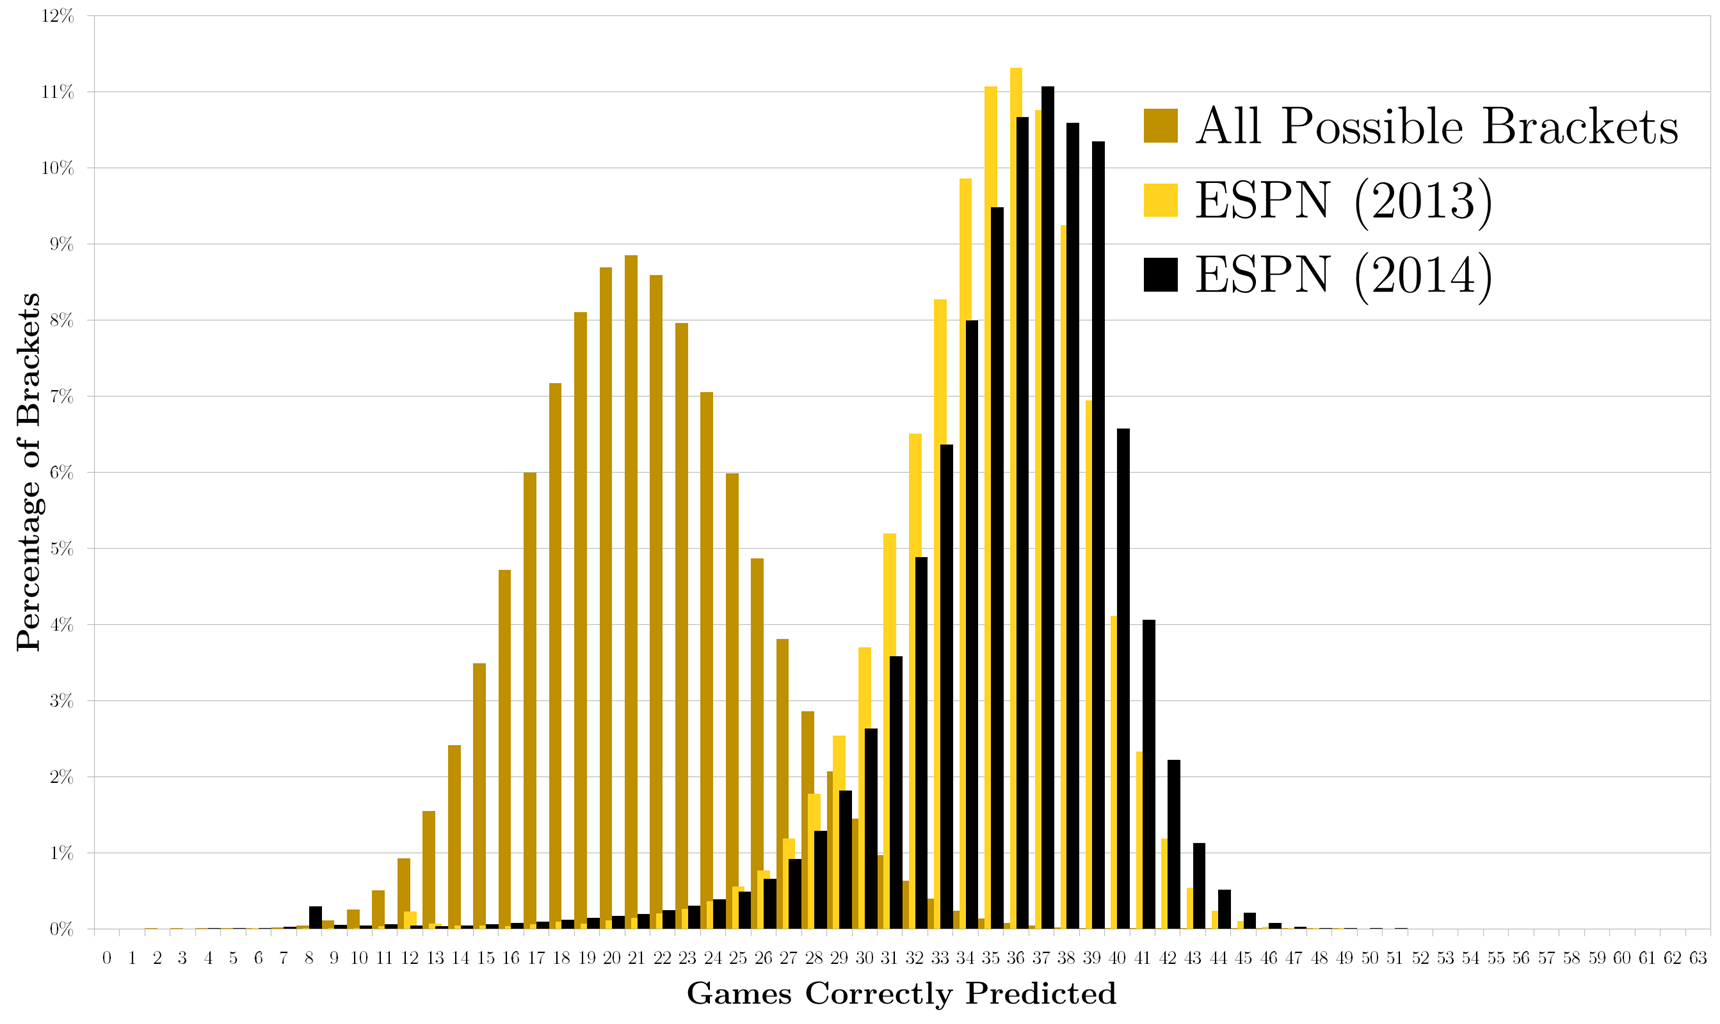
\includegraphics[width=7in]{distro2.png}
\caption{Distribution of the number of games correctly pick for all possible brackets along with the distributions of the 2013 and 2014 ESPN Tournament Challenge}
\label{distro}
\end{figure*}

\subsection{Tempo-Free Statistics}

Traditionally in basketball, team and player statistics are averaged on a ``per-game" (PG) basis. As such, when looking at a stats page on the NCAA D-1 men's basketball website, one will find the abbreviations PPG (points per game),  OPP PPG, (opponent's points per game), APG (assists per game), and RPG (rebounds per game).  In recent years, however, there has been a shift by some away from these statistics in exchange for statistics that are independent of a team's tempos. 

The tempo of a basketball team is defined by the number of possessions a team has in a game. In NCAA D-1 men's basketball, each team has 35 seconds to shoot the ball and at least hit the rim; otherwise, the ball is turned over to the other team.  There are some teams that will pass the ball frequently looking for the best open shot and use nearly all of this time, but there are others that try to make the first available shot they have. As such, the number of possessions in a single 40 minute game can be dramatically varied. 

There are many arguments for tempo free statistic. First, basketball can be viewed as a turn based game where every possession ends with points, a missed shot, or a turnover before possession is transferred to the other team. Consequently, the offense would like to convert possessions into as many points as possible while the defense would like to prevent the other team from doing so. Second, since 40 minutes is not necessarily long enough to collect an adequate sample of possessions over which to average. Third,  the number of possessions in the game will differ. Therefore,  it is easier to compare teams on the per possession basis, or in other words, to use tempo-free statistics.   

For example, suppose Player A and Player B both average 20 points per game, but the tempo of their respective teams is 60 and 80 possessions per game. This means Player A is averaging 2 points every 6 possessions while Player B is only averaging 2 points every 8 possessions. Put this way, it is easier to see that Player A is more effective at converting possessions to points than Player B.

This idea of making statistics that are independent of a team's tempo, or tempo-free statistics, have been championed by analysts like Ken Pomeroy, who runs the site \url{kenpom.com}. This site provides tabulated tempo-free statistics such as the adjusted offensive efficiency(AdjOE), the adjusted defensive efficiency(AdjDE), and the Pythagorean expectation(Pyth). To help explain and familiarize these statistics, they are defined below along with the highest and lowest occurrence in the 2014 tournament. It is important to note that all of these statistics are defined as some sort of estimate against an average D-I team. What this is saying is that assuming that if a D-I team throughout the course of the season has faced a good sampling of D-I teams, then what they have accomplished is a good approximation for how they would do against the average D-I team. For example, The adjusted offensive efficiency is an estimate of the number of points scored a team would have against the average D-I defense per 100 possessions. In the 2014 tournament, Creighton, a number three seed, had the highest adjusted offensive efficiency at 125.7 points scored per 100 possessions while Coastal Carolina, a 16 seed, had the lowest at 97.3 points scored per 100 possessions. The adjusted defensive efficiency is an estimate of the number points allowed by a team against the average D-I offense per 100 possessions by the defense. Arizona, a one seed, had the best adjusted defensive efficiency of 86.9 points allowed per 100 possessions while Eastern Kentucky, a 15 seed, had a adjusted defensive efficiency of only 108.3 points allowed per 100 possessions. 

Finally, the Pythagorean expectation is a descriptive statistic that combines the adjusted offensive efficiency and the adjusted defensive efficiency and is an estimate a team's expected winning percentage against an average D-I team. In general, a Pythagorean expectation is calculated using the following formula:

\[
Pyth = \frac{\mbox{points scored} ^ 2}{\mbox{points scored} ^ 2 + \mbox{points allowed} ^ 2}
\]

It gets its name from its resemblance to the Pythagorean equation. As each sport keeps score in dramatically different ways, each uses different measures of offense and defense as well as different exponents. For the Pythagorean expectations tabulated on \url{kenpom.com}, the formula is

\[
Pyth = \frac{AdjOE^{11.5}}{AdjOE^{11.5} + AdjDE^{11.5}}
\]

where the exponent of 11.5 was fitted by Ken Pomeroy using the 2002 - 2013 seasons' data. As a percentage, Pythagorean expectations are bounded between 0 and 1. Arizona had the highest Pythagorean expectation at .9540 and with Coastal Carolina have the lowest at .3552.


\subsection{Current Methods}

There are many current methods that are used to try to correctly predict the results of the tournament. The first, and simplest, is the idea of ``picking chalk." This is a term in sports betting that has its origins back to the day that betting odds where written on chalkboards. As more people placed bets on the favorite-to-win, the odds would be erased and changed to  reflect the moving position. This frequently left the name of the favored-to-win obscured in the resulting chalk dust. As such, ``chalk" refers to picking the favorite-to-win. In this case, by definition of the seeding process,  it means always choosing the highest seeded team to win.  As the tournament bracket explicitly gives ranks to the teams, using this method yields a unique bracket that is called the ``chalk" bracket. While this is a very simple idea, it usually fares well in small bracket pools. 

The other method compared in this paper is the Log5 method, created by Bill James for use in baseball.  Log5 is a method of estimating the probability one team will beat another based on their true winning percentages. A true winning percentage is the percentage of games a team \emph{should} win if they were to play sufficiently many games as to average out any amount of luck. It is suspected that the name of the Log5 method comes from the resemblance  the formula has to the logit function and the fact that it uses the assumption that the average performance is assumed to be $p_L \equiv .500$. The below formulation would be an estimate for team a beating team b.

\[
Log5_a = \frac{\frac{p_a}{1-p_a}}{\frac{p_a}{1-p_a} + \frac{p_b}{1-p_b} * \frac{p_L}{1-p_L}} = \frac{p_a (1 - p_b)}{p_a (1 - p_b) + p_b (1 - p_a)}
\]

The Log5 method does have some very useful properties. 

\begin{itemize}
\item $Log5_a + Log5_b = 1$.
\item If $p_A = 1$, then $Log5_a = 1$.
\item If $p_A = 0$, then $Log5_a = 0$.
\item If $p_A = p_B$, then $Log5_a = Log5_b = .5$.
\item If $p_A = 1/2$, then $Log5_a = 1-p_B$.
\end{itemize}


One thing that is of importance to note is that the Log5 method relies on knowing each team's ``true" winning percentage. Currently, this is being provided in college basketball by the Pythagorean expectation. This paper seeks to calculate a more accurate winning percentage to use in the Log5 method in order to predict game outcomes.


\section{Methodology}

When looking at the probability that a bracket will occur, there are two stances that can be taken. The first is to calculate the probability of a team advancing to the next round conditional on all possible games that could occur. While this is the most mathematically sound, it is much more computationally intensive to model. It also has the potential to make some strange results. For example, it is possible for teams that have a less than 50\% chance of winning in one round to advance to next round if their chances of winning (or losing) in the next round are extreme ($P \leq .05 \mbox{ or }  P \geq .95)$. In this case, intuition would state that picking a team to advance when it is predicted to lose the first game would be a poor choice. However, the likelihood of a bracket where this team does advance may be greater than for brackets where this team is not chosen to advance, thereby possibly predicting an upset. This method will be referred to as the conditional method.

The second way is to calculate the probability based on the teams that are actually in the match, independent of what has happened or what will happen latter. In other words, this method looks at each of the 63 games as independent. In this approach, the individual game is predicted based on that game alone. Then, the winners are advanced to play in another independent game. This has the benefit of always choosing the team with the highest probability of winning the game, but this also means that it is less likely to predict upsets. This method will be referred to as the independent method.

\subsection{k-Nearest Neighbor}

The k-Nearest Neighbor is a method of regression used to determine a value of a property based on the value of this property in $k$ neighbors. For the purpose of this paper, the property to be determined is the outcome of a game against an opponent, with the neighbors being opponents that were faced during the regular season.  Based on the outcome of the previous matches, a distance-weighted value was added to a win or loss parameter for the closest $k$ previous opponents. Proximity was determined simply using the Manhattan distance between team's Pythagorean expectations. This process is then repeated for the opponent. These results are aggregated to determine a winning percentage that can be used in the Log5 method. Below is the formula for team a with W and L representing the win and loss parameters mentioned above.

\[
p_{a} = \frac{W_a + L_b}{W_a + W_b + L_a + L_b}
\]
To help illustrate this procedure, the first round game from the 2014 tournament between fifth seeded Cincinnati and twelfth seeded Harvard will be used as an example.  After the regular season, Cincinnati finished the season with a win-loss record of 27-6 ($Pyth = .8701$) and Harvard finished 25-4 ($Pyth = .8402)$. With the Log5 method using the Pythagorean expectations, one would give Cincinnati a 56\% chance of beating Harvard. However, if the 10 closest matches ($k=10$) are examined for each team, then Cincinnati is 5-5 with Harvard being 8-2. With the Log5 method using the this procedure, one would give Harvard a 73\% chance of beating Cincinnati.  When the game was played, Harvard did in fact upset Cincinnati.

In order to determine the appropriate value for $k$, backtesting was done on the 2003 - 2013 tournaments. The data for these seasons were provided by Ken Pomeroy. For each tournament, $k$ values of between 3 and 30 were used and applied in both the conditional and independent methods. The goodness of the $k$ value was measured by the taking number of games correctly predicted using the $k$ value  minus the number of games correctly predicted using the traditional log5 with Pythagorean expectations. This was done to normalize the data in a sense, as there were some years that were much easier to predict than others and could have potentially skewed the results.

\section{Results}

Upon backtesting, it was determined that a $k$ value of 25 performed the best for both the conditional and independent methods, with the conditional method doing slightly better over the span tested.

These results were then applied to 2014 bracket. In \ref{tab_2014}, the results for the experiment can be seen, as well as some prominent results for comparison. The National bracket compiles brackets submitted to ESPN by using a team's selection to advance on an individual's bracket as a vote for that team to advance on the compiled bracket. This is in contrast to the average ESPN bracket, which is the average number of games correctly predicted on 1.5 million of the nearly 12 million submitted brackets, rounded up.  

It should be noted that $k=25$ was, upon running all other $k$ values for 2014, the best value for 2014.

In the future, different and more comprehensive methods of proximity could be fitted to help improve the overall accuracy.



\section{Conclusion}

\begin{table}[!t]
\caption{Results for 2014 Tournament}
\label{tab_2014}
\centering

\begin{tabular}{|c|c|}
\hline
Bracket & Games Correct\\
\hline
\hline
The National Bracket & 39\\
Average ESPN Bracket & 36\\
``Chalk" & 39\\
Conditional kNN (k=25) & 42\\
Independent kNN (k=25) & 40\\
Log5 (Both Methods) & 38\\
President Obama & 40\\

\hline
\end{tabular}
\end{table}

These results were then applied to 2014 bracket. In \ref{tab_2014}, the results for the experiment can be seen, as well as some prominent results for comparison.

While for 2014 the k-Nearest Neighbor approach has produce slightly better results, it does not seem to be statistically better than the other methods.



\section{Future Works}

As a large $k$ value in general appeared to be preferred over small $k$ values, an extension of this work using a pure distance-weighted nearest neighbor algorithm where all points are always included could be promising. The data of past seasons could then be used to do a regression of the distance formula. 


\section*{Acknowledgment}


The authors would like to thank Ken Pomeroy for providing them with the data necessary for this research and Sara Hagmann for her help in proofing this paper.



\end{document}
